\documentclass[12pt, letterpaper]{article}
\usepackage[hyphens]{url}
\usepackage{breakurl}
\usepackage[pdftex]{graphicx}
\usepackage[left=1in,top=1in,right=1in,bottom=1in,head=.5in,foot=.5in]{geometry}
\usepackage{setspace}

%\usepackage{caption}
\usepackage{subcaption}
%\usepackage[small,compact]{titlesec}
\usepackage{listings}
\usepackage{listings}
\usepackage{color}
\lstnewenvironment{fileName}{%
\lstset{%
        basicstyle=\ttfamily,
        breaklines,
    }%
}{%
}

\title{Security Audit of Safeplug}
\author{Annie Edmundson and Anna Kornfeld Simpson}

\begin{document}

\maketitle

\section{Introduction}
\label{sec:intro}

User privacy is becoming increasingly important as more Internet users realize how vulnerable they are to attackers and eavesdroppers.  This has been exacerbated by the current news about the NSA's surveillance of the Internet~\cite{nsa}.  Unfortunately, the average Internet user is not aware of how to protect themselves against malicious users.     



\section{Goals}
\label{sec:goals}
TODO: Annie
In this project, we would like to do a security audit of the Safeplug and investigate the following questions.  How does the box pick which relay node on the Tor network to connect to?  What kind of authentication goes on between the box and the Tor node?  Does it use the same route of Tor relays every time?
Safeplug claims to offer in-box ad-blocking.  How does this work and does it remove any functionality?  Is there an easy way to whitelist things without turning Safeplug off entirely?

What are the configurations on the box?  Is it clear to users what information is being hidden and what information is being leaked?  The website talks a lot about IP addresses and warns users to clear cookies \cite{safeplug}, but is that sufficient to preserve anonymization across all web traffic (including Flash or Javascript supercookies that might not be cleared when cookies are cleared)?  Can user anonymity be leaked by a user’s behavior while still using the Safeplug?  What else must a user do in addition to using the Safeplug to further preserve anonymity?

Safeplug can act as a relay in the Tor network \cite{techreview}; how would widespread use of the box affect the Tor network?


\section{Procedure}
\label{sec:procedure}
TODO: Anna
Safeplug is not open source, which makes a security audit much more challenging.  This leads to a debate on where a user will put his/her trust.  Despite not having the source code, we hope to get a Safeplug, set it up via their website, and use Wireshark to capture traffic and see what happens.  Wireshark allows us to capture and analyze network data \cite{wireshark}.  We are interested both in the communication between the clients and the Safeplug and between the Safeplug and the outside world. 

\section{Results}
\label{sec:results}
\subsection{User Experience}
\label{sec:ux}

Before setting up and using the Safeplug device, we read a variety of news articles as well as opinions through the Tor mailing list~\cite{tormailinglist}.  There were many thoughts on the Terms of Service and the option to use the device as a Tor relay node; this inspired us to start our analysis with these items.  

\subsubsection{Terms of Service}
\label{tos}
Safeplug's Terms of Service are interesting because they are controlling, yet the product they are for is a device for anonymization.  The first section of the Terms of Service explains how to agree to them:

\begin{quotation}
``You must agree to these TOS before you can use the Service. You can agree to these TOS by: a) actually using the Service, or b) clicking a box that indicates you agree to the Service, where such a box is made available to you.'' \cite{safeplug}
\end{quotation}

This is worth noting because option b) described above did not exist in any part of the setup process for Safeplug.  The Terms of Service continues by notifying readers that Pogoplug can change them any time they wish:

\begin{quotation}
``Pogoplug may update or change these TOS from time to time and recommends that you review the TOS on a regular basis at www.pogoplug.com/safeplug. You understand and agree that your continued use of the Service after the TOS has changed constitutes your acceptance of the TOS as revised. '' \cite{safeplug}
\end{quotation}

Most Safeplug users will likely not read the Terms of Service once, let alone on a regular basis; therefore, most users will be blind to any changes.  It is also interesting that these Terms of Service are only accessible through a small link at the bottom of the Safeplug website \cite{safeplug}; specifically, there is no documentation, including the Terms of Service, in the package that the device was shipped in.  Further along in the Terms of Service, the makers of Safeplug were sloppy when they wrote:

\begin{quotation}
``Pogoplug includes several open source components in the Software. You agree to abide by the terms of the relevant licenses, as may be updated by Pogoplug from time to time at http://pogoplug.com/home-en-developers-open-source.html. '' \cite{safeplug}
\end{quotation}

The link included is a dead link and takes the user to a web page with a 404 error.  This lack of attention to detail or respect for open source licenses does not put Pogoplug in a good light.  In fact, the Tor mailing list noted this particularly, since Tor is an open source project \cite{tormailinglist}.  The last section of the Terms of Service that stood out described Pogoplug's policy on updates:

\begin{quotation}
``As part of the Service, you may from time to time receive updates to the Software from Pogoplug that may be automatically downloaded and installed to your applicable device. These updates may include bug fixes, security enhancements or improvements, or entirely new versions of the Software. You agree that Pogoplug may automatically deliver such updates to you as part of the Service. '' \cite{safeplug}
\end{quotation}

This should raise a red flag for users because they may not know when the software in their device is being changed or what it is changing to.  While Safeplug makes many claims about providing anonymity, users are simply putting their trust in a different entity, namely Pogoplug.

\subsubsection{Tor Relay Node Option}
One of Safeplug's configurations is the use of the device as a Tor relay node in the Tor network.  When the device is initially setup, the default setting is to not use it as a relay node.  

One of our concerns is how understandable this setting is to the average Internet user.  The settings page describes Tor in an extremely basic way, as shown in Figure~\ref{fig:funnydesc}, but describes the functionality of a Tor relay node in a much more technical manner.  This description is shown in Figure~\ref{fig:relaydesc}.  If the majority of users can only understand the simpler description, then they likely won't understand the description of a Tor relay node.  This could be a problem if users simply decide not to do anything with that setting (i.e. don't change the setting to use Safeplug as a relay node).  Then there would be a large increase in use of the Tor network, yet most of the users are not giving back to it.

\begin{figure}[htb]
\begin{center}
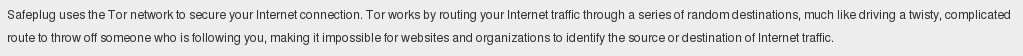
\includegraphics[width=\textwidth]{funnydesc.png}
\caption{This is a figure.}
\label{fig:funnydesc}
\end{center}
\end{figure}

\begin{figure}[htb]
\begin{center}
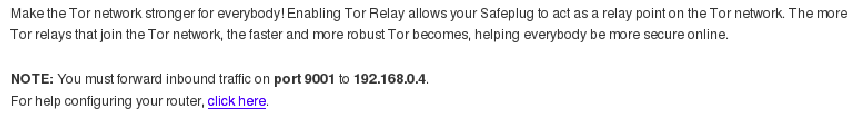
\includegraphics[width=\textwidth]{relaydesc.png}
\caption{This is a figure.}
\label{fig:relaydesc}
\end{center}
\end{figure}

This could easily be remedied; Safeplug should choose a target audience and have consistent descriptions.  The best option is to explain the Tor network and the functionality of a Tor relay node at the same level, preferably a level that normal Internet users can understand.  This increases the chances that users will run their Safeplug as a relay node.

\subsubsection{Internet Use}
\label{inetuse}
{\bf Setting up Safeplug.} The first step was to plug Safeplug into our router and activate our device.  Our instructions are shown in Figure~\ref{fig:instructions}.  We followed them, activated our device, and then ended on the configuration page.  The configuration page has a combination of platforms and browsers, with a different set of proxy configuration instructions for each one.  It is interesting to note that the only platform options were: OSX, Windows, Android, and iOS.  Figure~\ref{fig:proxyconfig} shows our configuration. 

\begin{figure}[htb]
\begin{center}

\includegraphics[width=\textwidth]{instructions}
\caption{This is a figure.}
\label{fig:instructions}
\end{center}
\end{figure}

\begin{figure}[htb]
\begin{center}
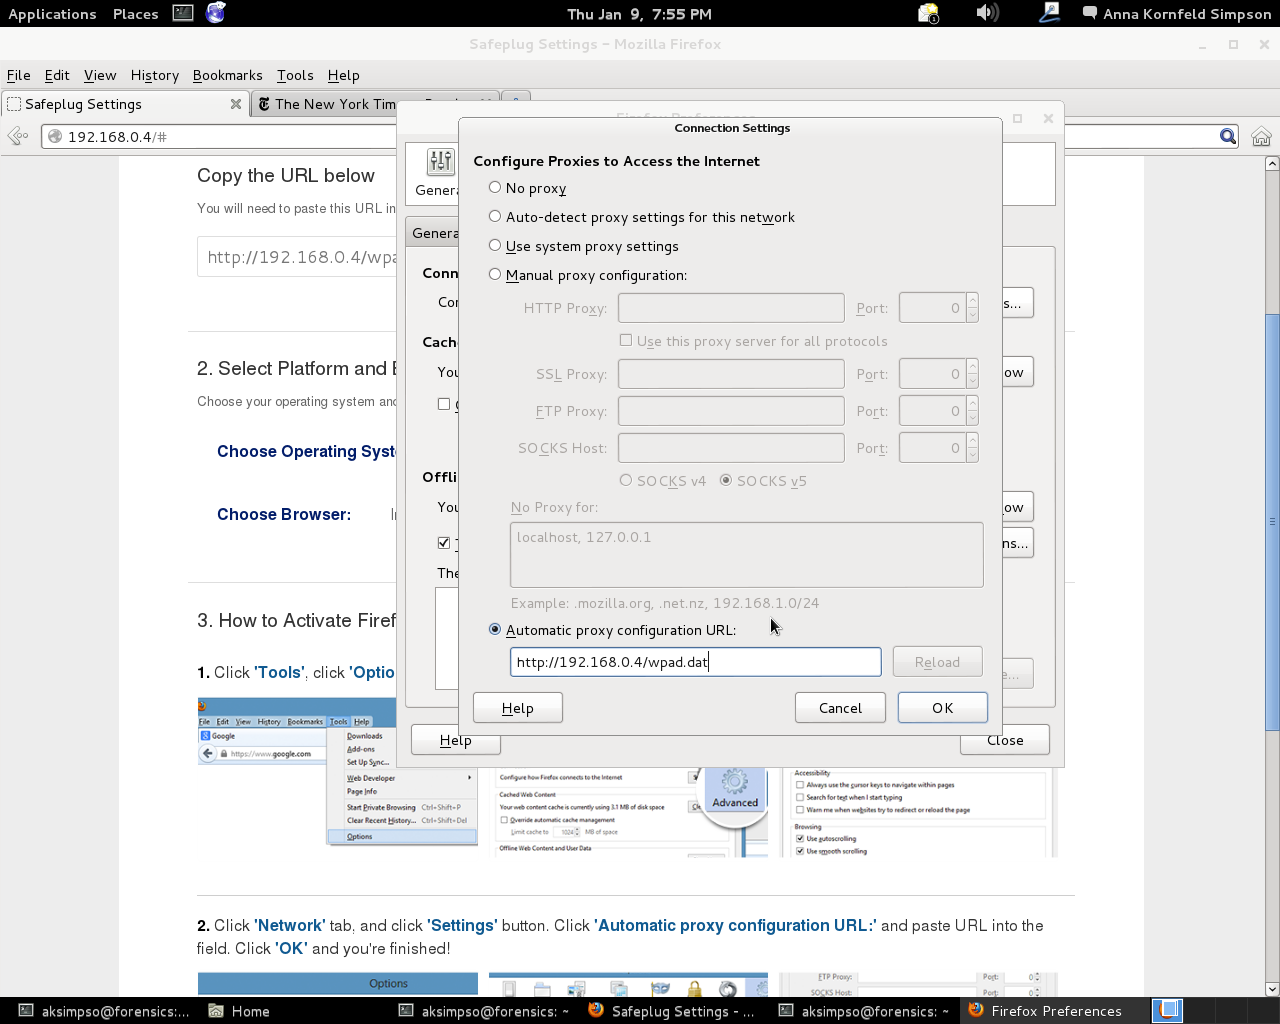
\includegraphics[width=\textwidth]{proxyconfig}
\caption{This is a figure.}
\label{fig:proxyconfig}
\end{center}
\end{figure}

After we finished our configuration, we were taken to our settings.  This page is shown in Figure~\ref{fig:settings}.  This allowed us to turn on/off Tor, add whitelisted websites, turn on/off ad-blocking, and turn on/off the ability of our device to be a relay node.  

\begin{figure}[htb]
\begin{center}
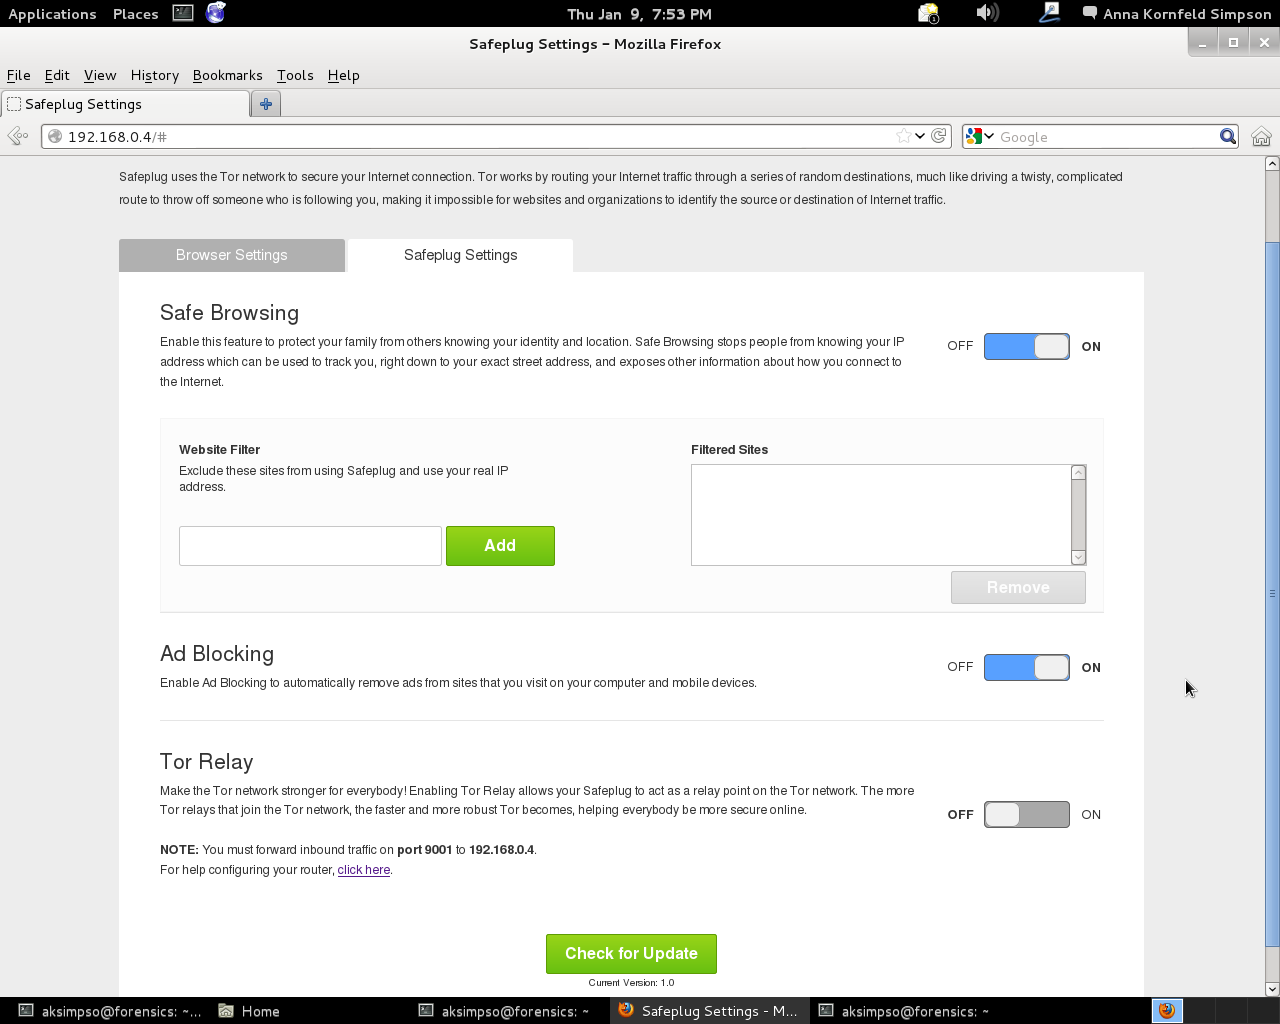
\includegraphics[width=\textwidth]{settings}
\caption{This is a figure.}
\label{fig:settings}
\end{center}
\end{figure}

{\bf Using the Internet.} Figure~\ref{fig:before} shows what a web page looks like before turning Tor and ad-blocking on, while Figure~\ref{fig:after} shows the same website after turning Tor and ad-blocking on.  Both of these figures show our IP address in the top right corner; due to the change in IP address we can see that our traffic is being routed through Tor.  

\begin{figure}[htb]
\begin{center}
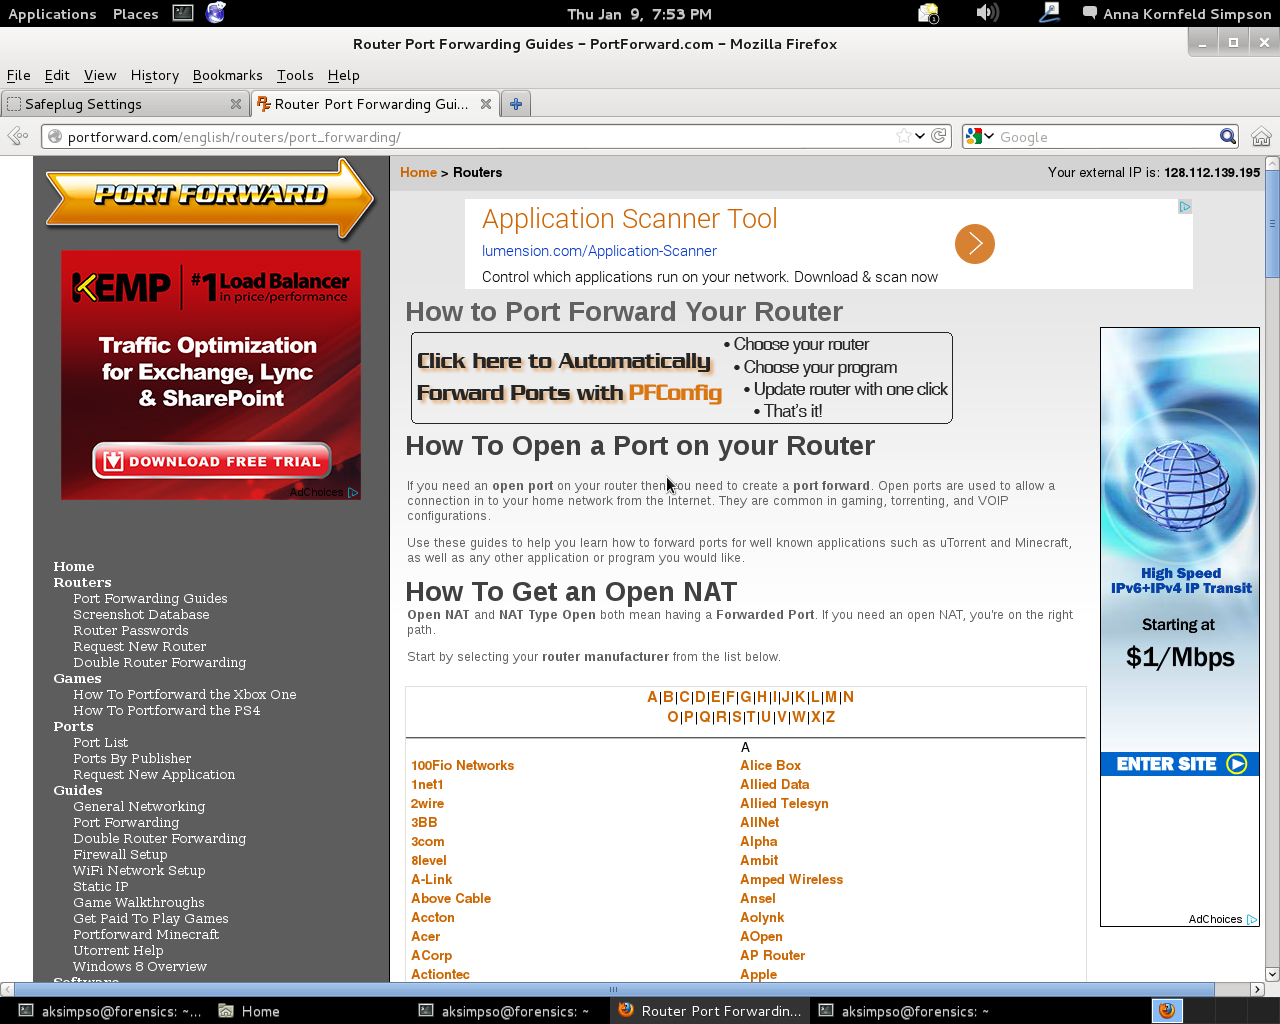
\includegraphics[width=0.5\textwidth]{before}
\caption{This is a figure.}
\label{fig:before}
\end{center}
\end{figure}

\begin{figure}[htb]
\begin{center}
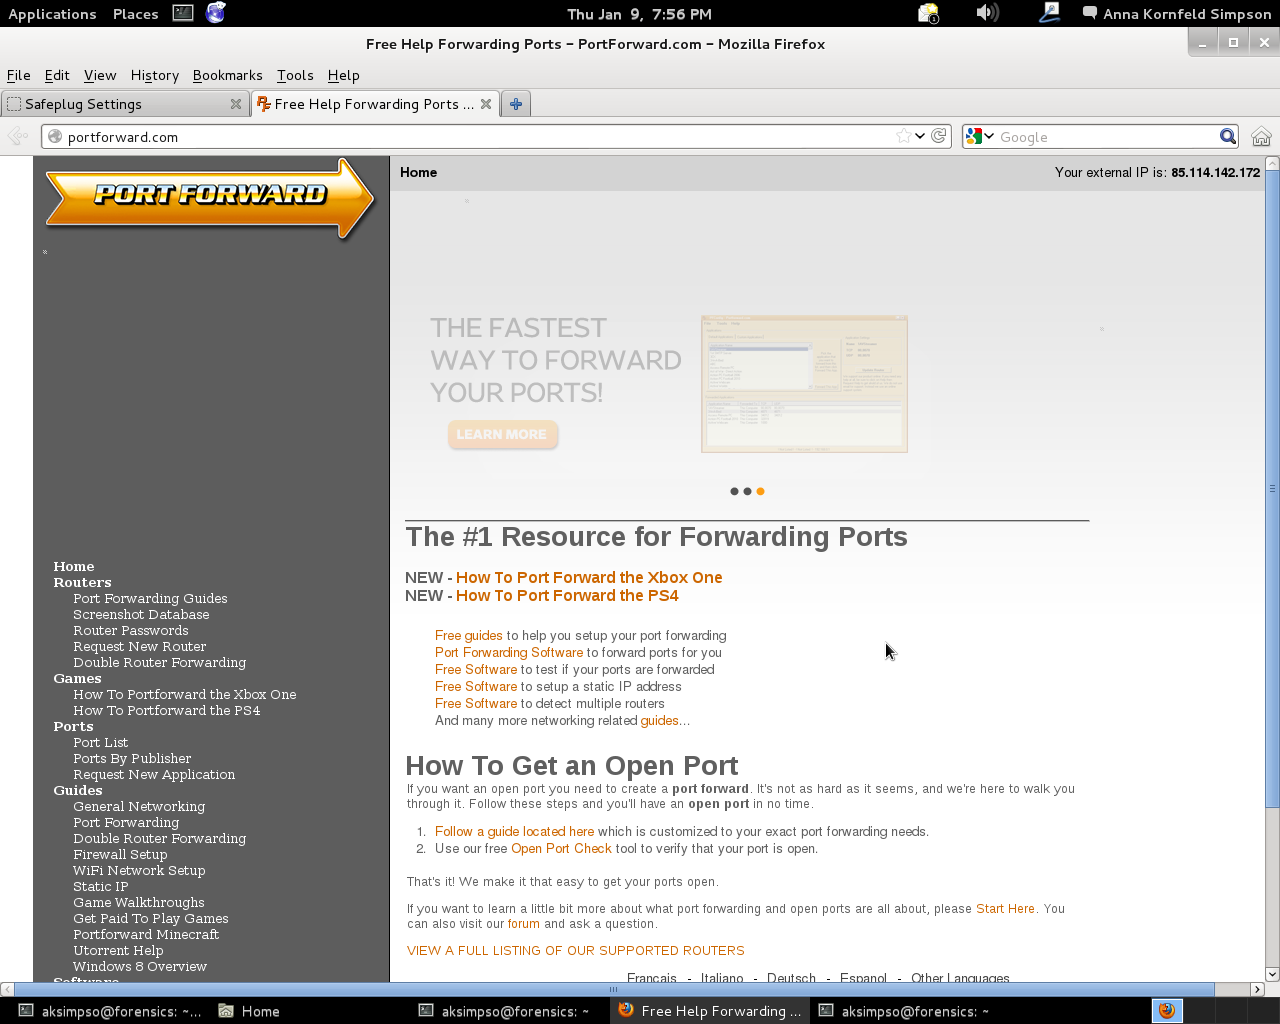
\includegraphics[width=0.5\textwidth]{after}
\caption{This is a figure.}
\label{fig:after}
\end{center}
\end{figure}

Next, we wanted to see how usable this would be to a normal Internet user.  A user would probably decide not to use Safeplug if they couldn't read their web pages (if they weren't in their native language), or if they couldn't log into their accounts (some web sites will lock a user out if they try to login from multiple countries in a short time period).  While browsing the Internet, we experienced some pages in German and Swedish, which is expected with Tor; if a user is not familiar with Tor, then they may just get frustrated and stop using Safeplug altogether.  We were also prompted with the page in Figure~\ref{fig:funnygoogle} when we tried to log into our Google account. 

\begin{figure}[htb]
\begin{center}
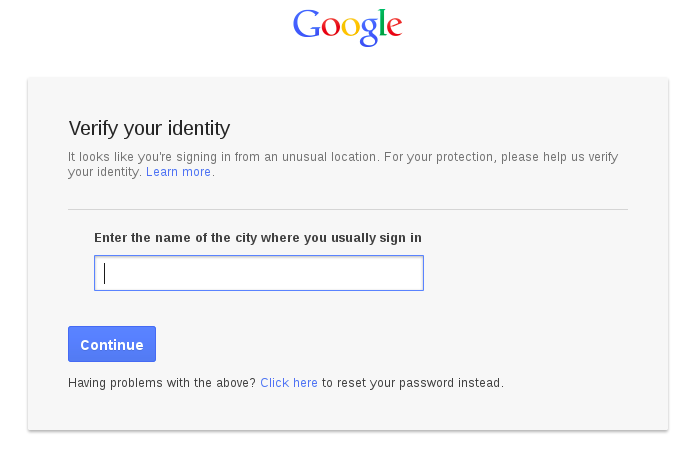
\includegraphics[width=0.5\textwidth]{funnygoogle}
\caption{This is a figure.}
\label{fig:funnygoogle}
\end{center}
\end{figure}

{\bf Cookies.}  While browsing the Internet, we logged into a Google Account in a tab, and then subsequently went to a website that had the Google+ logo in a different tab.  When we clicked on the Google+ logo, it remember who we are; so we can confirm that we still have first-party cookies.  We experienced the same situation with Facebook and its corresponding ``like'' button.

\subsection{Teardown}
\label{sec:tear}
We opened up the Safeplug device to look at the internals.  Figure~\ref{fig:top} shows the top of the board and Figure~\ref{fig:bottom} shows the bottom.  We identified an SD card slot, Lan transformer, and Ethernet transceiver on the top of the board.  On the bottom, we found flash memory and the integrated circuit.

\begin{figure}[htb]
\begin{center}
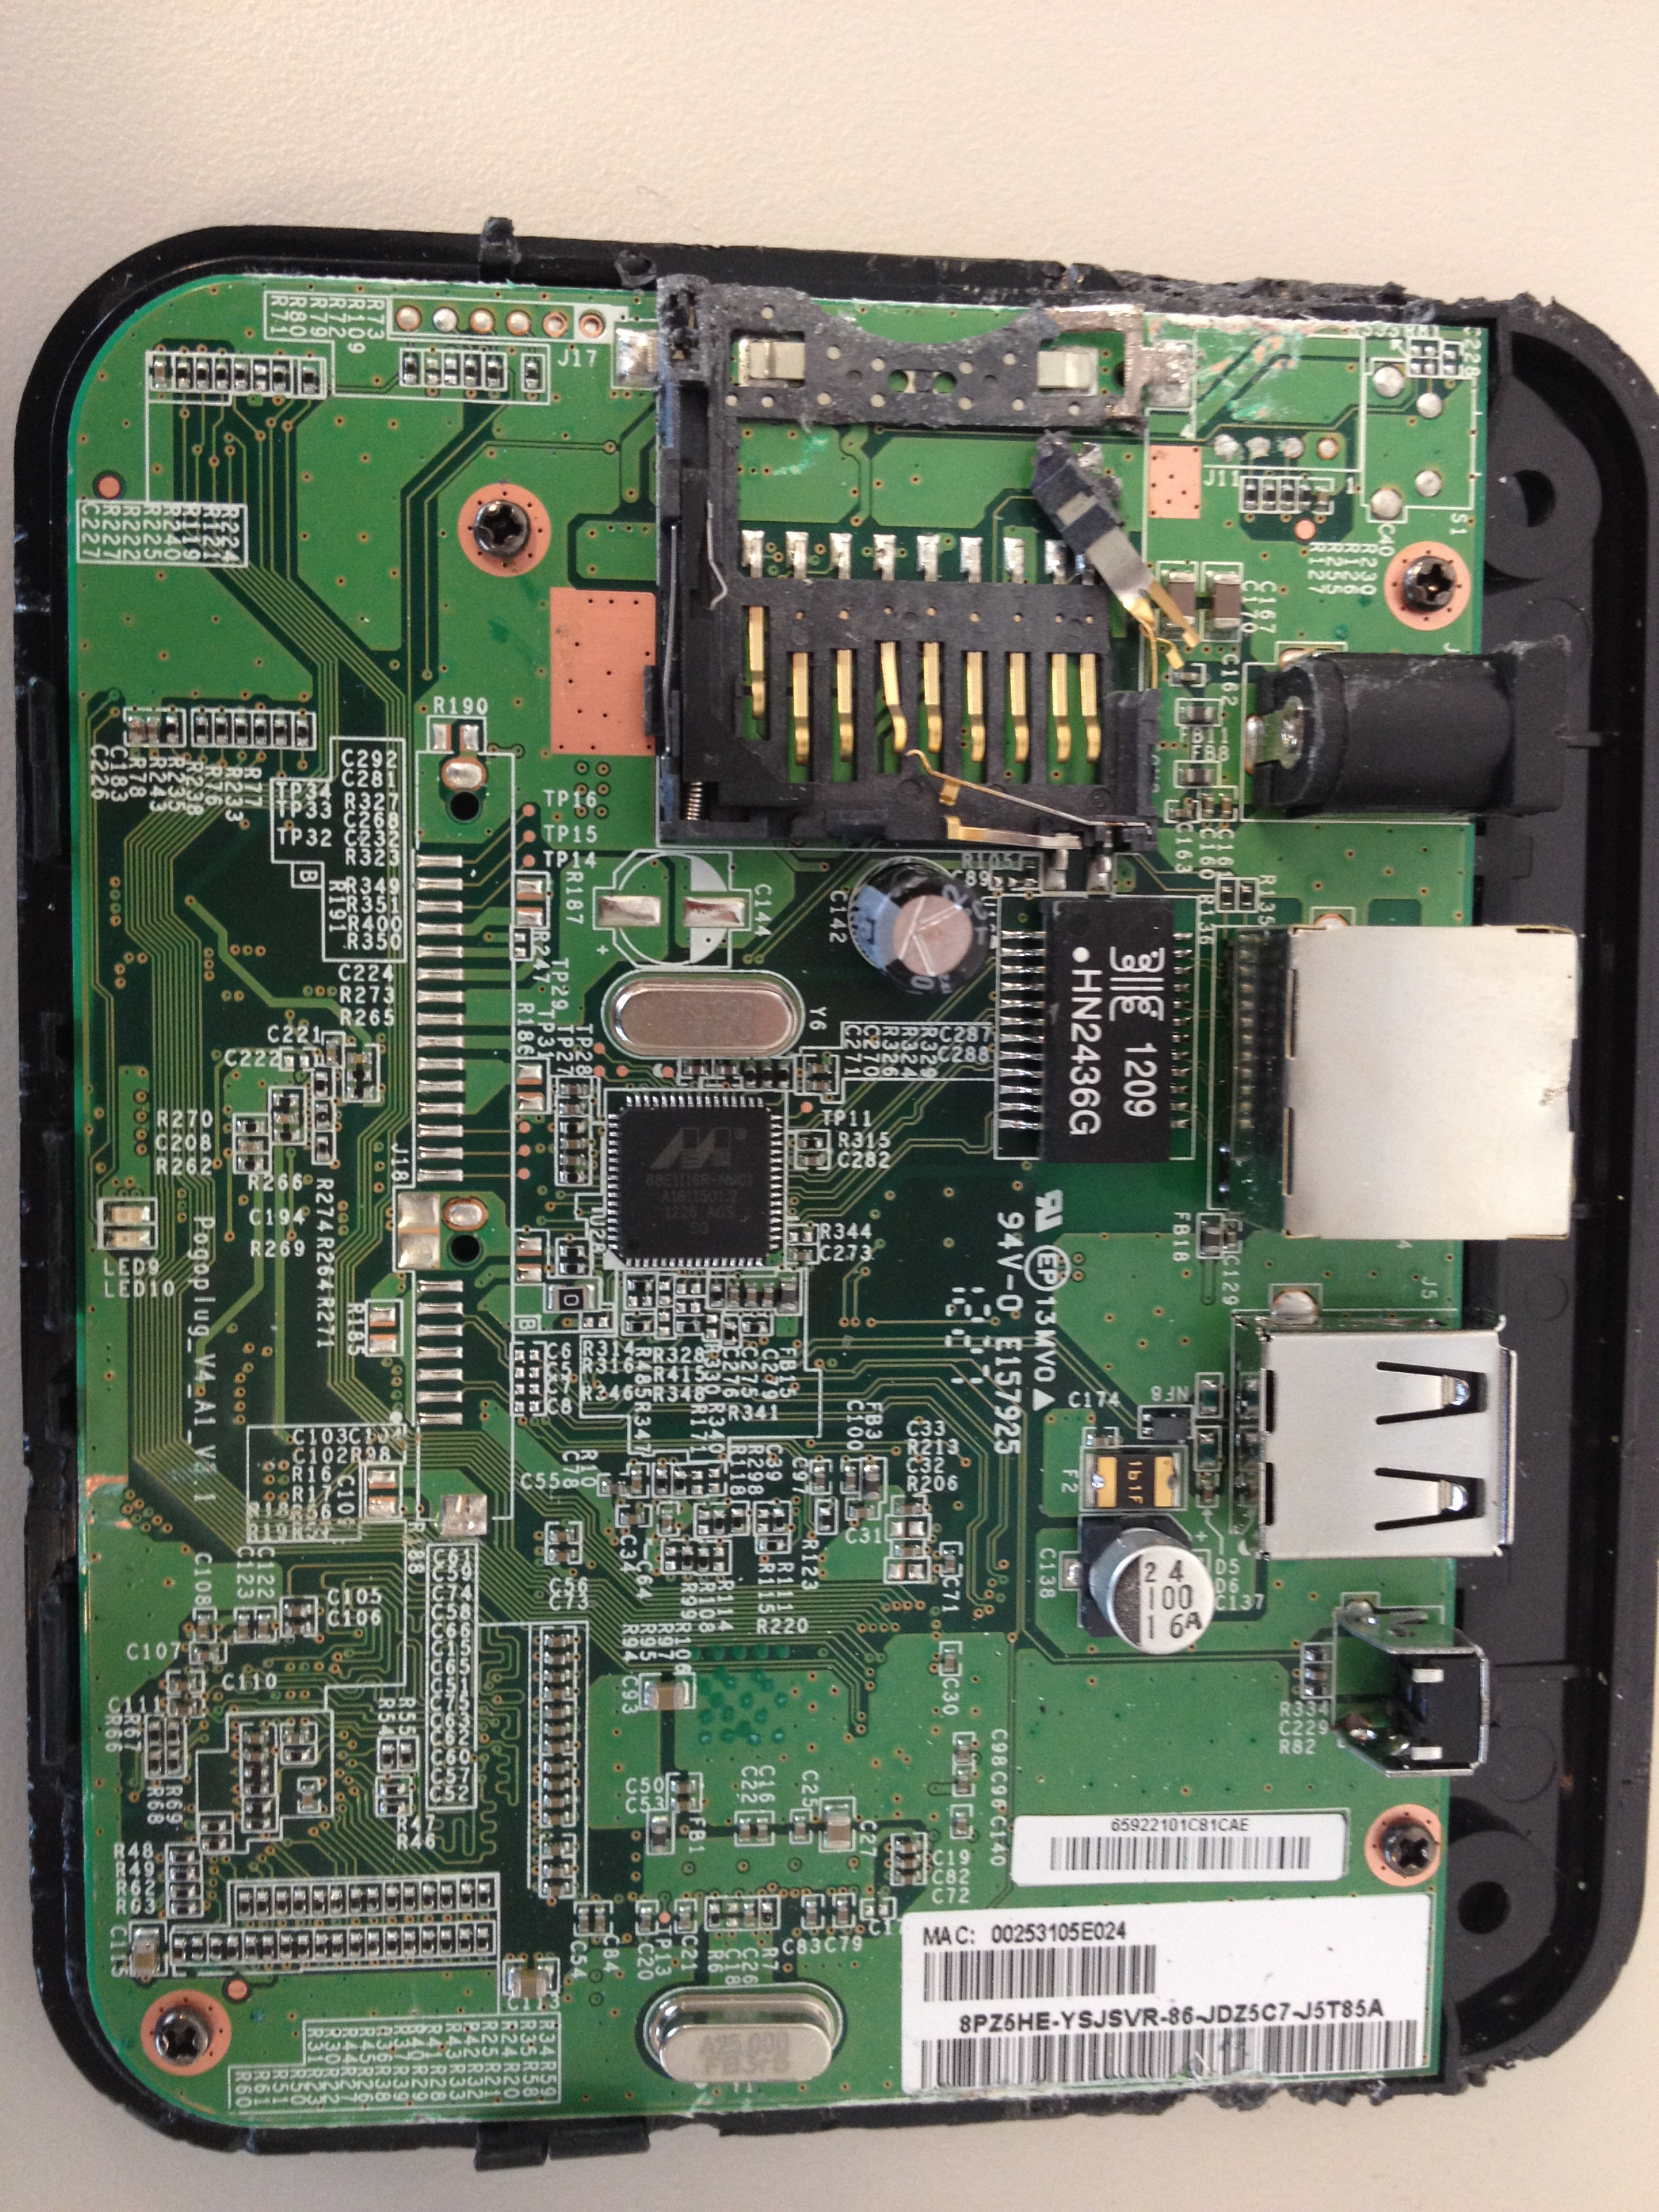
\includegraphics[width=0.25\textwidth]{safeplug_top}
\caption{This is a figure.}
\label{fig:top}
\end{center}
\end{figure}

\begin{figure}[htb]
\begin{center}

\includegraphics[width=0.25\textwidth]{safeplug_bottom}
\caption{This is a figure.}
\label{fig:bottom}
\end{center}
\end{figure}

\subsection{Traffic Analysis}
\label{sec:traffic}

\subsubsection{Initial Plugin Behavior}
Before allowing the Safeplug box to be connected to the outside world, we attached it to the home connection setup described in Section \ref{sec:proc} and captured traffic for a few minutes on the local network.  From visual inspection (Figure \ref{redlight}), there was certainly something trying to access the internet and displaying an error on its failure.  

\begin{figure}[htb]
        \centering
        \begin{subfigure}[b]{0.3\textwidth}
                
\includegraphics[width=\textwidth]{redlight.jpg}
                \caption{Safeplug box when only connected to the local network.}
                \label{redlight}
        \end{subfigure}%
        \quad %add desired spacing between images, e. g. ~, \quad, \qquad etc.
          %(or a blank line to force the subfigure onto a new line)
        \begin{subfigure}[b]{0.4\textwidth}
          \centering
          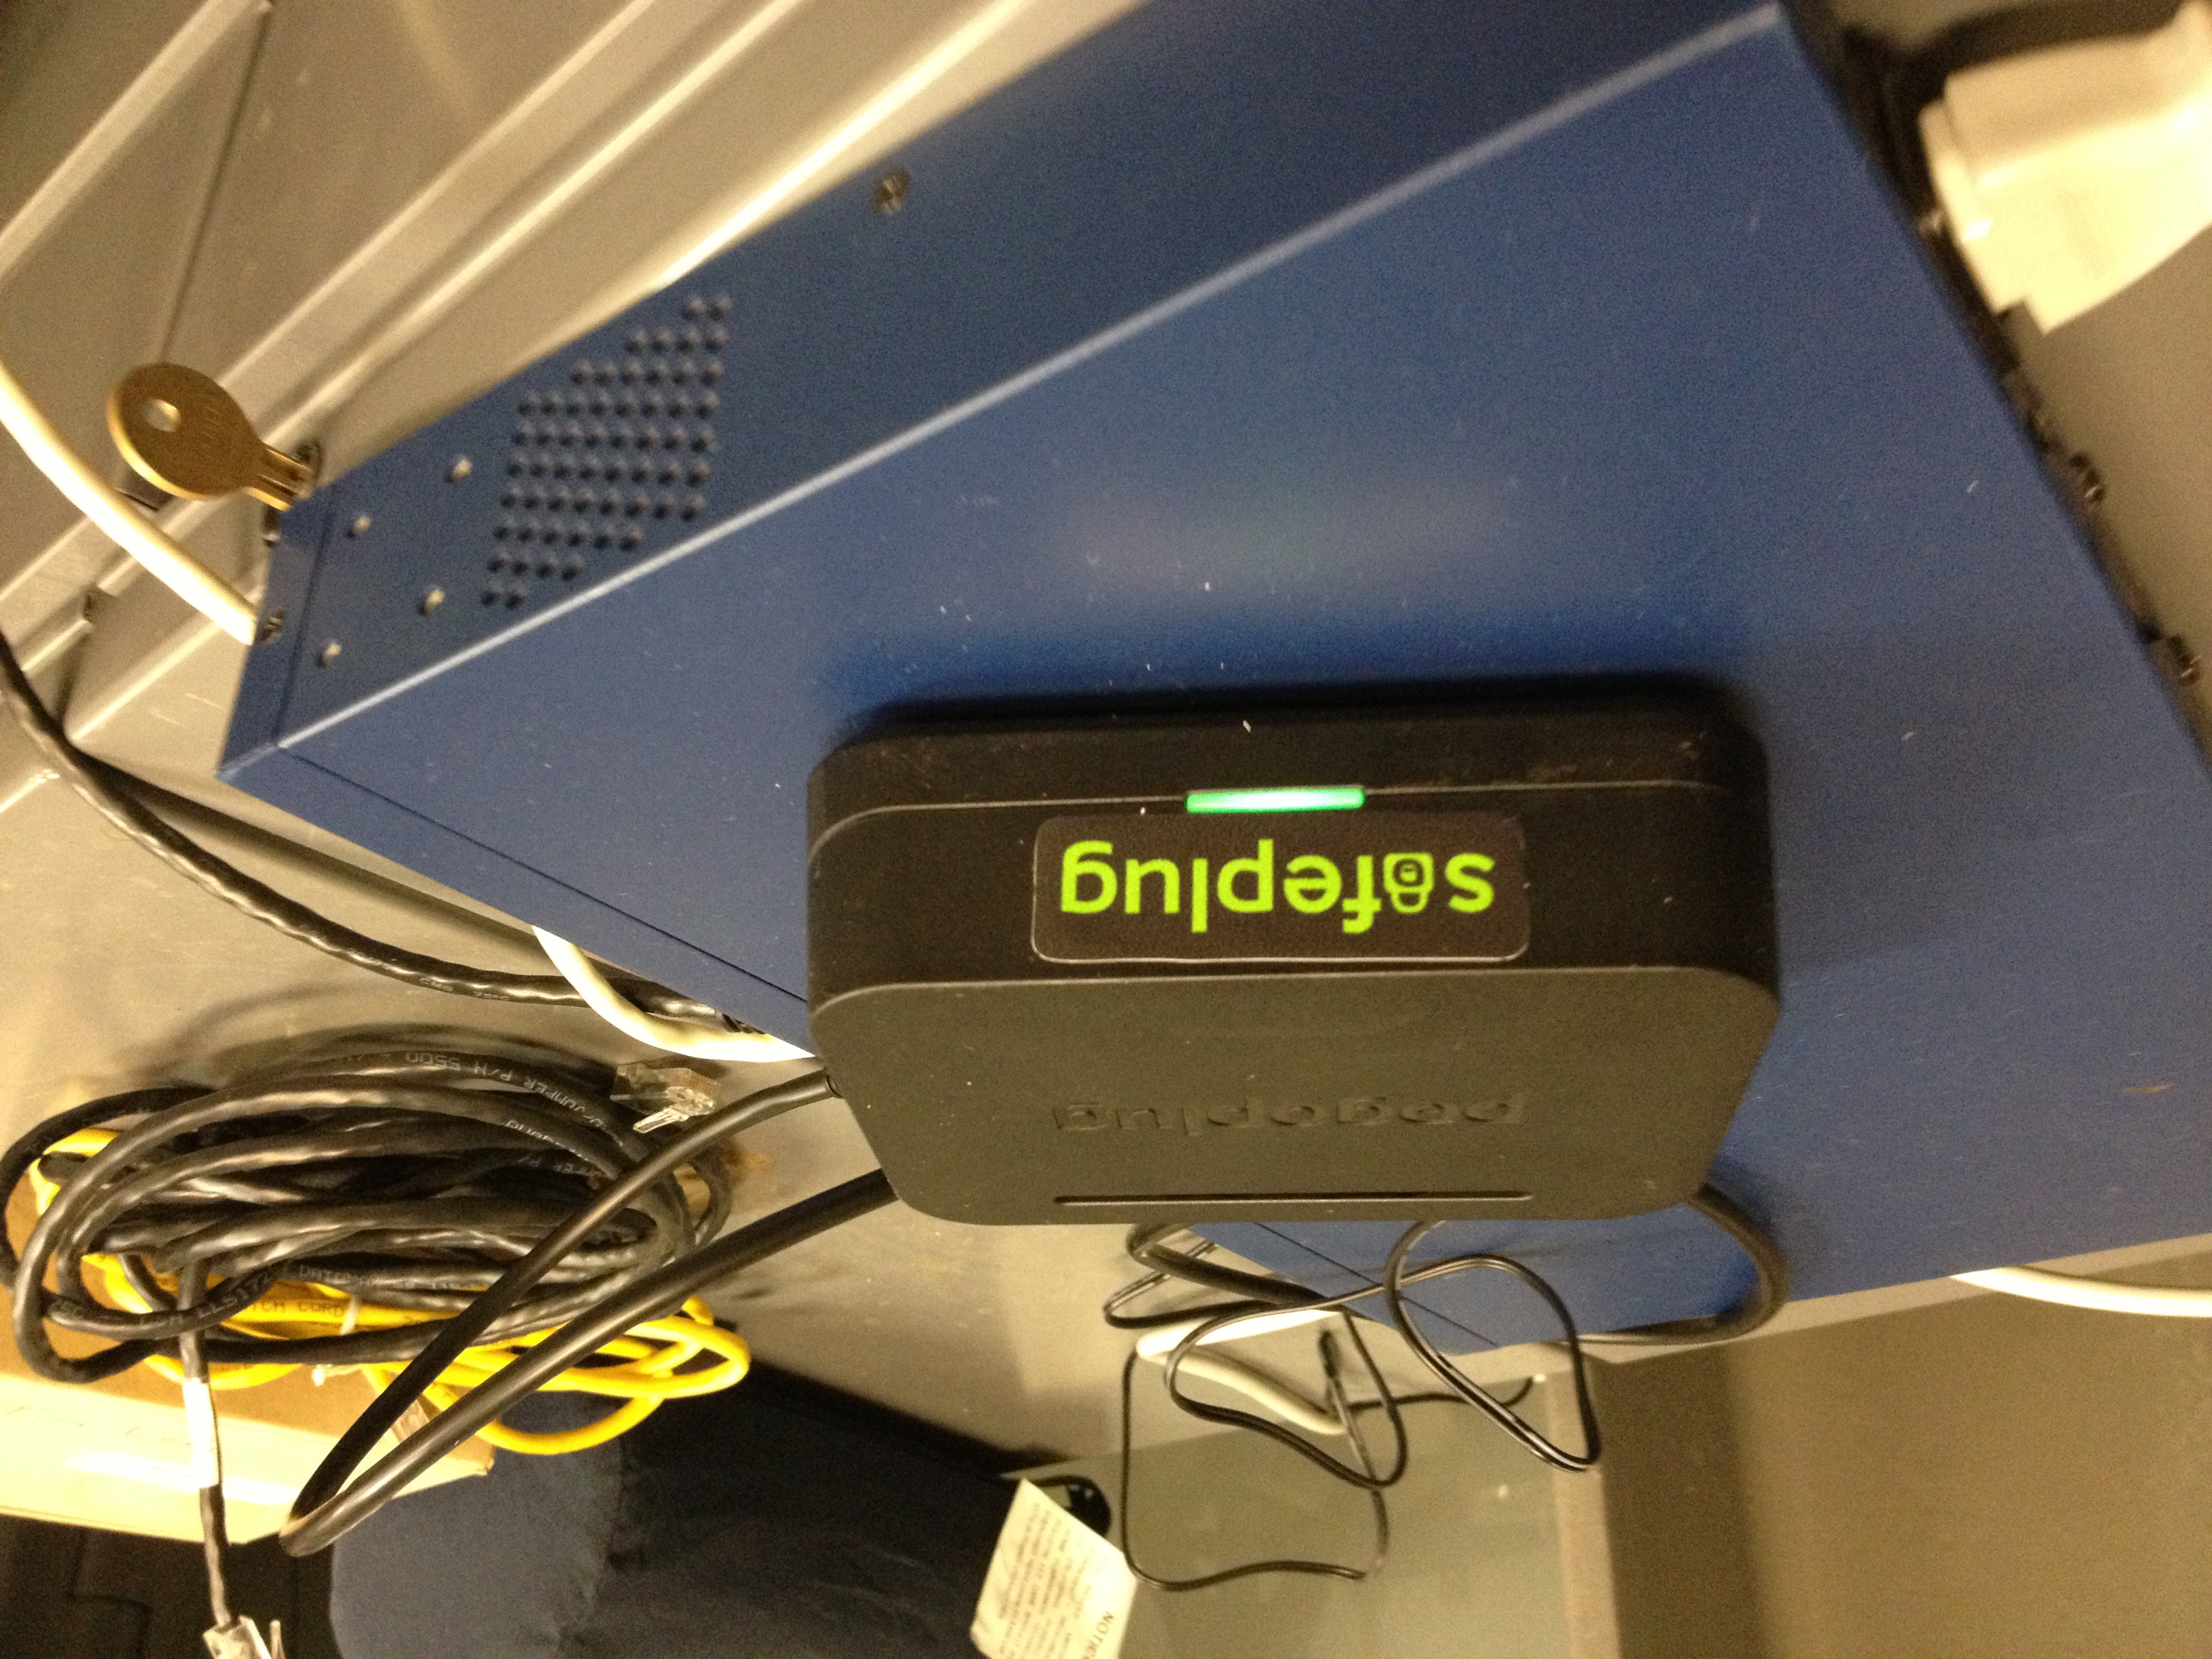
\includegraphics[width=.66\textwidth,angle=180]{greenlight.jpg}
                \caption{Safeplug box after connection to the internet, regardless of whether Tor was enabled.}
                \label{greenlight}
        \end{subfigure}
        \caption{Safeplug box during initial setup prior to an internet connection and after activation from the Pogoplug website.}
        \label{fig:lights}
\end{figure}

Analysis of the TCP dump showed that the Safeplug box repeatedly queried the local DNS server for two items: \url{pogoplug.com} and the NIST standardized time.  The first query for the time was to \url{www.nist.gov}, and subsequent queries included \url{nist1-chi.ustiming.org}, \url{nist1-ny.ustiming.org}, \url{time-nw.nist.gov}, and \url{nist1.symmetricom.com}.  Queries about pogoplug were mostly for \url{service.pogoplug.com} but after that set was tried \url{secure.pogoplug.com} was attempted once.  While it was only connected to the local network, we also did a scan of all the ports of the Safeplug and only port 80 was open.

\subsubsection{Activation and Update Traffic}
\label{updatetraf}
After establishing the initial update behavior, we connected the other end of our homemade router back to the internet and captured traffic on both the network interfaces. As we had seen previously, the first effort of the Safeplug was to query for \url{service.pogoplug.com} and connect, and the send a POST/XML request to that server containing a 16 byte numerical string of type \verb!nid!, \verb!0x0! as \verb!flags!, and a field called \verb!pingdata! with length of 423 bytes and undiscernable contents.  In future work, we hope to explore the contents of this automatic connection with the Pogoplug servers to discover what information is being passed along. 

The client computer then navigated to the Pogoplug website to complete the activation processes.  Each step of the process resulted in both TCP and UDP traffic between the Safeplug box and the pogoplug servers.  Most interesting was the update step in which the Safeplug box knew to request a script from \url{<update server IP>/svc/upgrade/safeplug\_switch.sh}.  Since this operation occured over normal HTTP, we were able to use \verb!curl! to recover the same script and examine it to discover the contents of the upgrade.

The upgrade script shows (and the network traffic confirms) that the box downloads and installs the following \verb!.tgz! files: 
\begin{fileName}
safeplug_lighttpd, safeplug_lighttpd_config, safeplug_wget, safeplug_certs, safeplug_gohelper, safeplug_tor, safeplug_tor_config, safeplug_privoxy, safeplug_privoxy_config
\end{fileName}
  Each file is compared to an MD5 hash before being unzipped and installed.  Details about the software found on the Safeplug are discussed in Section \ref{software}.  After the two lighttpd installations, a process called \verb!hbplug! is killed and lighttpd is started.  After the certs are downloaded, the current \verb!/usr/local/ssl! is overwritten with the new certs.  The \verb!go\_helper! is added to the \verb!/opt/xce/sbin! folder, and contains binary files with names related to update and upgrade (which we hope to decompile in future work).

After completing the installations, a default Safeplug configuation file is written with use of Tor set to 1.  (More information about the configuration in Section \ref{spconfig}.)  Finally, the old \verb!rcS! file in \verb!/etc/init.d! is replaced with commands to start lighttpd, tor and privoxy, and the LED is set to green as shown in Figure \ref{greenlight} after the completion of the upgrade. This means that the green LED indicates an up-to-date, internet-connected Safeplug, rather than anything about the use of TOR.

\subsubsection{Traffic After Activation}
After the activation and the configuration of the Safeplug as a proxy, all traffic was through the Tor network.  The Safeplug connected to a directory to learn about different relays and seemed to cycle through a small set around the world for different connections.  This demonstrates that Tor is working as expected.  If there is any ``phone-home'' being done by the device after Tor has been turned on, then it is doing so through the Tor network.


\subsection{Gaining Access through SSH}
\label{sec:SSH}
    \subsubsection{Accessing the Device}
    Safeplug runs an RPC server that allows the enabling of SSH access via HTTP. SSH instructions for Cloud Engine's other device (Pogoplug) are widely available online and an email in the Tor-talk mailing list confirms that the instructions are the same (although the Pogoplug support staff note that SSH access breaks the warranty!) \cite{ceadmin}:
\begin{fileName}
curl --data ``'' http://<IP-of-Safeplug>/svc/xspctrl/enableSSHD
ssh root@<IP-of-Safeplug>
password: ceadmin
\end{fileName}

Obviously having a publically available root password means that SSH can be done effectively without authentication.  We tried the SSH procedure twice, once before the internet connection and activation, and once afterwards.  Before the activation and update procedure, SSH was not available.  The simple \verb!Hbplug! software on the box could not accept this RPC call.  However, once the box was updated and had lighttpd installed, the SSH procedure was available and we could download the contents of the root filesystem for analysis.

    \subsubsection{Software on the Safeplug}
\label{software}
As would be suspected from the analysis of the update script described above in Section \ref{updatetraf}, the installed software is in \verb!/opt/xce! and includes lighttpd, privoxy, and tor.  Lighttpd is an open-source webserver, which is serving the settings page on the device - the project's description mentions ``security, speed, compliance, and flexibility [... while being] designed and optimized for high perfomance environments'' \cite{lighttpd}.  Privoxy is a ``non-caching web proxy with advanced filtering capabilities for enhancing privacy, modifying webpage data and HTTP headers, controlling access, and removnig ads and other obnoxious Internet junk'' and it specifically advertises its ``flexible configuration'' \cite{privoxy}.  Privoxy is also open source.  All three pieces of software appear to be there with default configuration files (with all appropriate citations and comments present).  The Safeplug uses its own configuration files to determine how these pieces of software are set up and used.
    
    \subsubsection{Configuration on the Safeplug}
    \label{spconfig}
The Safeplug configuration files can be found in \verb!/opt/xce/etc! and include \verb!sp.conf! and \verb!sp_version! and \verb!sp_torexceptions!.  The first contains all of the important details from the configuration page (whether to use Tor, whether to be a relay, whether to adblock) as well as a hidden option about whether to be an exitrelay for the Tor network.  This is not documented anywhere on the site, so enabling this option would likely require SSH access to discover it, thereby breaking the warranty, but it is interesting that this option is available.  The version file is likely used for updates, and the exceptions file is used by the privoxy configuation to control the whitelist of sites not to connect to via Tor.

These configuration files are read by the scripts in \verb!/opt/xce/etc/init.d! which enable lighttpd, privoxy, and tor.  As expected, Privoxy looks at the Tor, adblock and exceptions configurations, and Tor reads the \verb!sp.conf! file to set which Tor configuration file (regular, relay or exitrelay) to use.

\subsection{Attacking the RPC Capability}
As we discovered while enabling SSH, the Safeplug has a remote procedure call (RPC) capability.  This is a script called \verb!xspctrl! found in \verb!/opt/xce/html/svc! and it contains more options than just SSH enabling.  Particularly, functional calls to this script include enable and disable for all of the Safeplug settings, including Tor, ad block, and Tor relay.  None of them require any arguments in the POST string.

\begin{figure}[htb]
\begin{center}
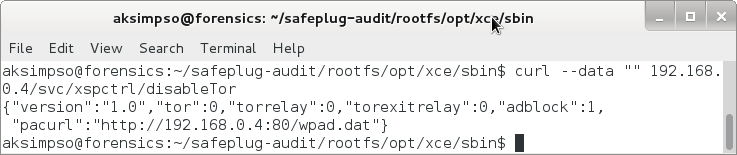
\includegraphics[width=.75\textwidth]{disabletor}
\caption{Disabling Tor as an insider attack.}
\label{disable}
\end{center}
\end{figure}

\subsubsection{Insider Attack}
Since the RPC server does not perform any kind of validation or authentication on the settings strings, it would be easy for anyone inside the local network to send a command and change the settings, for example to disable Tor or adblocking.  All the attacker would need to know is the IP of the device.  It does not even require SSH or discovering the (publically available) root password, or the user's new root password if they have been well-informed and adept enough to change it.  Figure \ref{disable} shows an example of this attack.

This attacker could also be any kind of device on the local network, or the local gateway if it is compromised.  The NSA ``Spymall'' catalog leaked in December shows tools for compromising a number of different devices and home routers are traditionally insecure \cite{spymall}.  It is easy to imagine any malicious party, not just one with the resources of a government, (although governments might be some of the most interested parties in attacking a Tor proxy) compromising the gateway and using that access make a disabling RPC call into the Safeplug.  This would occur silently from the perspective of a client unless the happen to check the Settings page for the Safeplug.  Instead, the client would continue browsing with a belief that they are protected by their use of the Tor network, while in fact any external adversary can track their traffic.

This seems like a fairly important vulnerability and requires action from Pogoplug to fix.  Since the purpose of these RPC operations is unclear without access to more of the source code, it is possible that they could be disabled entirely.  If not, perhaps there is some authentication protocol that could be implemented.  The challenge of such a protocol from a user's point of view is that valid access would be infrequent so giving a user a password to remember would be a poor experience.


\subsubsection{Website Attack}
An external website can also perform this attack by returning a correctly formatted POST string.  This executes the same functionality as the Insider Attack, but the attacker does not need to be on the local network or know the IP address of the Safeplug.  Instead, the attacker (who could be any malicious actor with access to a web server) can just send a POST request to every IP in the common ranges of local addresses in home networks, 192.168.0.0/24 and 192.168.1.0/24.  We implemented this attack with less than 30 lines of Javascript code (See Appendix A).  The following steps are necessary for the attack to be successful:

\begin{enumerate}
\item Set up a web page with the crafted Javascript code, which will send a POST request of the following format to all addresses in the range: http://$<$IP address$>$/svc/xspctrl/disableTor (See Appendix A).
\item Send the malicious link to a user in the targeted private network.
\item Once the user clicks the link and loads the malicious site, the correctly formatted POST request will be sent to every IP address in the ranges.  
\item Tor is disabled silently.  The user must check or refresh her settings page to learn that Tor is turned off.  
\end{enumerate}  

This exploits the RPC server in the same manner that the Insider Attack does.  While this attack requires a greater amount of time because the local IP address of the Safeplug must be guessed via search, but the number of private address spaces is small, and the space likely to be occupied by a Safeplug on a home network is even smaller.  

The largest observed time to send requests to the 192.168.0.0/24 space was ~400 milliseconds; the entire attack costs ~800 milliseconds for sending request to both 192.168.0.0/24 and 192.168.1.0/24 ranges - even when the website was being loaded over Tor.  In the case of a private network in the range of 172.16.0.0/16, the attack took less than ~12 minutes (this generates script timeout warnings in most major browsers, which affects the timing of this attack).  This means that it would take a few hours to send requests to the full 172.16.0.0/12 range, which is commonly used in business networks.  The final private network space is 10.0.0.0/8 which is too large for an exhaustive search, but some simple optimization might make it feasible as well.  For example, using a GET request to get and parse the Safeplug settings page would allow the script to positively identify the safeplug and stop the search.  However, the 192.168.0.0/24 and 192.168.1.0/24 ranges are much more common in home networks; because Safeplug is geared towards home network use, in most cases the script will take less than a second, a trivial amount of time for the attacker to spend.  

In addition to disabling Tor, the attacker can modify any other settings on the device.  This includes: enabling/disabling Tor, enabling/disabling ad-blocking, enabling/disabling the use of the device as a Tor relay node [note: this requires the user to do additional setup], enabling/disabling the use of the device as an exit node (if it is already a relay).  Lastly, the attacker can also modify the user's whitelist of sites that should not be routed through Tor.  This whitelist attack is particularly dangerous because the change is silent and much harder for the user to notice the addition of a single website to the whitelist than a global loss of Tor.  (Removal of a webpage from the whitelist is likely to to cause usability problems and be more evident.)


\section{Related Work}
\label{sec:related}

To our knowledge, there has been no other study analyzing the security of Pogoplug's Safeplug device.  However there has been much prior research on the primary technology that the device uses: Tor.  Additionally, the security goals that Safeplug attempts to achieve have been previously studied in great detail; these include fingerprinting and cookies.  

{\bf Tor.} Prior security evaluations of the Tor network reveal a myriad of potential vulnerabilities.  A significant area of research on Tor relates to diversity of autonomous systems (ASes).  Feamster and Dingledine argue that a user's anonymity may be compromised by using geographically diverse ASes; when analyzing both sides of an anonymous path, it is more likely the same AS will appear in both sides of a long path than in a short path~\cite{feamster}.  Murdoch and Zielinski also argue against AS diversity.  They state that AS diversity does not improve security because traffic is routed through ASes at Internet exchange points (IXPs); therefore, an IXP can observe traffic that passes through multiple ASes~\cite{murdoch2}.  There has also been proven traffic correlation attacks that are efficient on the Tor network~\cite{murdoch, overlier}.  Johnson, Wacek, Jansen, Sherr, and Syverson evaluated Tor's security against reasonably realistic adversaries and contribute metrics that model security over time.  They found that in a period of six months, 80\% of all users may be deanonymized by a reasonably realistic Tor-relay adversary.  Johnson et al. take into account how the Tor network evolves over time when evaluating Tor's security~\cite{tor2}.  While Safeplug does not introduce or modify how Tor is used, it routes all traffic through the Tor network; Safeplug is also vulnerable to the attacks found in prior research on Tor.  

{\bf Fingerprinting.}  Website fingerprinting attacks as well as remote physical device fingerprinting attacks have shown they can identify users, even when specific defense have been used in order to prevent these attacks. Previous research has shown that web page fingerprinting attacks are possible~\cite{dyer, herrmann, panchenko}.  Cai, Zhang, Joshi, and Johnson introduced both a web page and website fingerprinting attack that defeats many recently proposed defenses, including cover traffic and randomized pipeling.  They find that their attack is successful 83.7\% of the time when the defense is the use of Tor; the success rate decreases to 52.2\% when the defense is the use of Tor, randomized pipelining, padding packets to 1500 bytes, and adding cover traffic at a 1:1 ratio~\cite{fingerprint1}.  These results can be extended to the security of Safeplug.  Because Safeplug uses only Tor to anonymize users, it may be susceptible to this fingerprinting attack.

{\bf Cookies} There has been much policy and technology debate around the topic of third-party web tracking.  Mayer and Mitchell survey recent policy and technology stances on web tracking; while tracking allows for free web content and innovation, it compromises a user's privacy~\cite{commercial2}.  They discuss the existence and use of stateful tracking by using ``supercookies.''  While many companies use cookies, there has also been work in developing privacy-preserving third-party services, such as Privad, Adnostic, and RePriv~\cite{guha, toubiana, fredrikson}.  

\section{Conclusion}
\label{sec:conclusion}
This security audit of Safeplug shows a few holes in their promises of complete security and anonymity, as might be expected when the device meets the real world.  The network analysis shows taht the device accesses Tor as expected, and without too much cost to user experience.  However, the vulnerability of SSH access and the RPC server are a cause for concern.  We plan to continue investigating the avenues of future work identified in this study.


\section{Acknowledgements}
We would like to express our gratitude to Josh Kroll for donating a lot of time and his computer to the routing effort.  We also thank whoever left the very nice set of screwdrivers on our desks!

This paper represents our own work in accordance with University regulations.

Anna Kornfeld Simpson and Annie Edmundson

\begin{thebibliography}{99}

\bibitem{spymall} Appelbaum et. al. ``Shopping for Spy Gear: Catalog Advertises 
NSA Toolbox'' \emph{Der Spiegel} 29 December 2013 \url{www.spiegel.de/internatio
nal/world/catalog-reveals-nsa-has-back-doors-for-numerous-devices-a-940994.html}

\bibitem{nsa} Arther, Charles.  ``NSA scandal: what data is being monitored and how does it work?'' \url{http://www.theguardian.com/world/2013/jun/07/nsa-prism-records-surveillance-questions}.

\bibitem{fingerprint1} Cai, Xiang, et al. ``Touching from a distance: Website fingerprinting attacks and defenses.'' \emph{Proceedings of the 2012 ACM conference on Computer and Communications Security (CCS)}, 2012.

\bibitem{ceadmin} Colleton, Lee. ``Fwd: SSH on Safeplug'' \emph{Tor-talk mailing list} 2 January 2014. \url{http://archives.seul.org/or/talk/Jan-2014/msg00003.html}

\bibitem{tor} Dingledine, Roger, et. al. ``Tor: The second-generation onion router.'' \emph{USENIX Security Symposium}, 2004.

\bibitem{dyer} Dyer, Kevin P., Coull, Scott E., Ristenpart, Thomas, and Shrimpton, Thomas.  ``Peek-a-boo, i still see you: Why efficient traffic analysis countermeasures fail.'' \emph{In Proceedings of the 33rd Annual IEEE Symposium on Security and Privacy}, 2012.

\bibitem{feamster} Feamster, Nick, and Dingledine, Roger.  ``Location Diversity in Anonymity Networks.''  \emph{In ACM Workshop on Privacy in the Electronic Society (WPES)}, 2004.

\bibitem{fredrikson} Fredrikson, M., and Livshits, B. ``Repriv: Re-envisioning in-browser privacy.'' \emph{In Proceedings of the 2011 IEEE Symposium on Security and Privacy}, May 2011.

\bibitem{guha} Guha, S., Cheng, B., and Francis, P. ``Privad: Practical privacy in online advertising.'' \emph{In Proceedings of the 2011 USENIX Symposium on Networked Systems Design and Implementation}, April 2011.

\bibitem{bittech} Halfacree, Gareth. ``Pogoplug launches Tor-powered Safeplug'' \emph{bit-tech.net} 25 November 2013, \url{http://www.bit-tech.net/news/hardware/2013/11/25/pogoplug-safeplug/1}.

\bibitem{herrmann} Herrmann, Dominik, Wendolsky, Rolf, and Federrath, Hannes.  ``Website fingerprinting: attacking popular privacy enhancing technologies with the multinomial naive-bayes classifier.'' \emph{In Proceedings of the 2009 ACM workshop on Cloud computing security}.

\bibitem{tor2} Johnson, Aaron, et al. ``Users get routed: Traffic correlation on Tor by realistic adversaries.'' \emph{Proceedings of the 2013 ACM SIGSAC conference on Computer \& Communications Security (CCS)}, 2013.

\bibitem{dropbear} Johnston, Matt. ``Dropbear SSH.'' \url{https://matt.ucc.asn.au/dropbear/dropbear.html}

\bibitem{fingerprint2} Kohno, Tadayoshi et. al. "Remote physical device fingerprinting." Dependable and Secure Computing, IEEE Transactions on 2.2 (2005): 93-108.

\bibitem{lighttpd} Lighttpd. \url{http://www.lighttpd.net}


\bibitem{marvellhw} Marvell, ``88F6190 and 88F6192 Integrated Controller Hardware Specifications'' 2 December 2008. \url{http://www.marvell.com//embedded-processors/kirkwood/assets/HW_88F619x_OpenSource.pdf}

\bibitem{marvell} Marvell, ``Marvell 88F6192 SoC with Sheeva Technology'' 2009. \url{http://www.marvell.com//embedded-processors/kirkwood/assets/88F6192-003_ver1.pdf}

\bibitem{marvell2} Marvell, ``Marvell Alaska 88E1116R'' 2007. \url{http://www.marvell.com/transceivers/assets/Marvell-Alaska-88E1116R-Single-Port-GbE.pdf}

\bibitem{fourthparty} Mayer, Jonathan. ``FourthParty'' \url{http://fourthparty.info}

\bibitem{commercial2} Mayer, Jonathan R., and John C. Mitchell. "Third-party web tracking: Policy and technology." \emph{IEEE Symposium on Security and Privacy (SP)}, 2012.

\bibitem{gigaom} Meyer, David. ``Say hello to Safeplug, Pogoplug’s \$49 Tor-in-a-box for anonymous surfing'', \emph{GigaOm}, 21 November 2013. \url{http://gigaom.com/2013/11/21/say-hello-to-safeplug-pogoplugs-49-tor-in-a-box-for-anonymous-surfing/}.

\bibitem{murdoch} Murdoch, S.J., Danezis, G.  ``Low-Cost Traffic Analysis of Tor.'' \emph{In IEEE Symposium on Security and Privacy (Oakland)}, 2005.

\bibitem{murdoch2} Murdoch, S.J. and Zielinski, P.  ``Sampled Traffic Analysis by Internet-Exchange-Level Adversaries.'' \emph{In Privacy Enhancing Technologies (PET)}, 2007.

\bibitem{overlier} Overlier, L. and Syverson, P.  ``Locating Hidden Servers.'' \emph{In IEEE Symposium on Security and Privacy (Oakland)}, 2006.

\bibitem{panchenko} Panchenko, Andriy, Niessen, Lukas, Zinnen, Andreas, and Engel, Thomas.  ``Website fingerprinting in onion routing based anonymization networks.'' \emph{In Proceedings of the 10th Workshop on Privacy in the Electronic Society}, 2011.

\bibitem{pano} Panopticlick. \url{https://panopticlick.eff.org/}.

\bibitem{safeplug} Pogoplug. ``Safeplug'', \url{https://pogoplug.com/safeplug}.

\bibitem{privoxy} Privoxy. \url{https://www.privoxy.org}

\bibitem{schneier} Schneier, Bruce. ``Tor Appliance.'' \emph{Schneier on Security}, 27 November 2013. \url{https://www.schneier.com/blog/archives/2013/11/tor_appliance.html}.

\bibitem{techreview} Simonite, Tom. ``Online Anonymity in a Box, for \$49'', \emph{MIT Technology Review}, 21 November 2013. \url{http://www.technologyreview.com/news/521676/online-anonymity-in-a-box-for-49/}.

\bibitem{toubiana} Toubiana, V., Narayanan, A., Boneh, D., Nissenbaum, H., and Barocas, S. ``Adnostic: Privacy preserving targeted advertising.'' \emph{In Proceedings of the 2010 Network and Distributed System Security Symposium}, March 2010.

\bibitem{wired} Solon, Olivia. ``Safeplug makes it super-easy to harness Tor\'s anonymity at home,'' \emph{Wired UK}, 22 November 2013. \url{http://www.wired.co.uk/news/archive/2013-11/22/safeplug-tor}.

\bibitem{tormailinglist} Tor Mailing List.  \url{https://lists.torproject.org/pipermail/tor-talk/2013-November/031199.html}.

\bibitem{orbot} ``Tor on Android.'' \emph{Tor Project.} Accessed February 2014. \url{https://torproject.org/docs/android.html.en}

\bibitem{torproject} The Tor Project.  \url{https://www.torproject.org/}.

\bibitem{amorbot} The Tor Project. ``Orbot: Proxy with Tor.'' \emph{Google Android Market}. Accessed 7 February 2014, \url{https://play.google.com/store/apps/details?id=org.torproject.android}

\bibitem{wireshark} Wireshark, \url{http://www.wireshark.org/}. 

\end{thebibliography}


\newpage
\appendix
\section{\\Javascript for Website Attack} \label{App:AppendixA}
\definecolor{dkgreen}{rgb}{0,0.6,0}
\definecolor{gray}{rgb}{0.5,0.5,0.5}
\definecolor{mauve}{rgb}{0.58,0,0.82}

\lstset{frame=tb,
  language=Java,
  aboveskip=3mm,
  belowskip=3mm,
  showstringspaces=false,
  columns=flexible,
  basicstyle={\small\ttfamily},
  numbers=none,
  numberstyle=\tiny\color{gray},
  keywordstyle=\color{blue},
  commentstyle=\color{dkgreen},
  stringstyle=\color{mauve},
  breaklines=true,
  breakatwhitespace=true
  tabsize=3
}

\begin{lstlisting}
function go() { 
   var IP_SCANS = 255;
   var prefix = "http://192."
   var SECOND_START = 168;
   var SECOND_END = 168;
   var THIRD_START = 0;
   var THIRD_END = 1;
   var mydate = new Date();
   console.log(mydate.getTime());

   for (var i = SECOND_START; i <= SECOND_END; i++) {
      for (var j = THIRD_START; j <= THIRD_END; j++) {
         for (var k = 0; k < IP_SCANS; k++) 
         {
            var tryip = prefix +  i + "." + j + "." + k;
            var req = new XMLHttpRequest();
            req.open("POST", tryip + "/svc/xspctrl/disableTor", true);
            req.timeout = 1000;
            req.send();
         }
         // COMMENT THIS OUT BEFORE RUNNING LARGE SCANS!
         var mydate2 = new Date();
         console.log(mydate2.getTime() + " " + j);
      }
      var mydate = new Date();
      console.log(mydate.getTime() + " " + i);
   }
}
\end{lstlisting}

\end{document}
